\chapter{INSTALLATION}
\section{Obtain}

The {\iqist} is an open source free software package. We release it under the General Public Licence 3.0 (GPL). The readers who are interested in it can write a letter to the authors to request an electronic copy of the newest version of {\iqist}:
 
\noindent\colorbox{pink}{\parbox[r]{\linewidth}{\quad email: huangli712@gmail.com,}}
or they can download it directly from the public code repository:

\noindent\colorbox{pink}{\parbox[r]{\linewidth}{\quad http://bitbucket.org/huangli712/iqist.}}

\section{Uncompress}

The downloaded {\iqist} software package is likely a compressed file with zip or tar.gz suffix. The users should uncompress it at first. For examples:

\noindent\colorbox{pink}{\parbox[r]{\linewidth}{\quad \$ tar xvfz iqist.tar.gz.}}

\section{Direcrory structures}
\begin{figure}[ht]
\centering
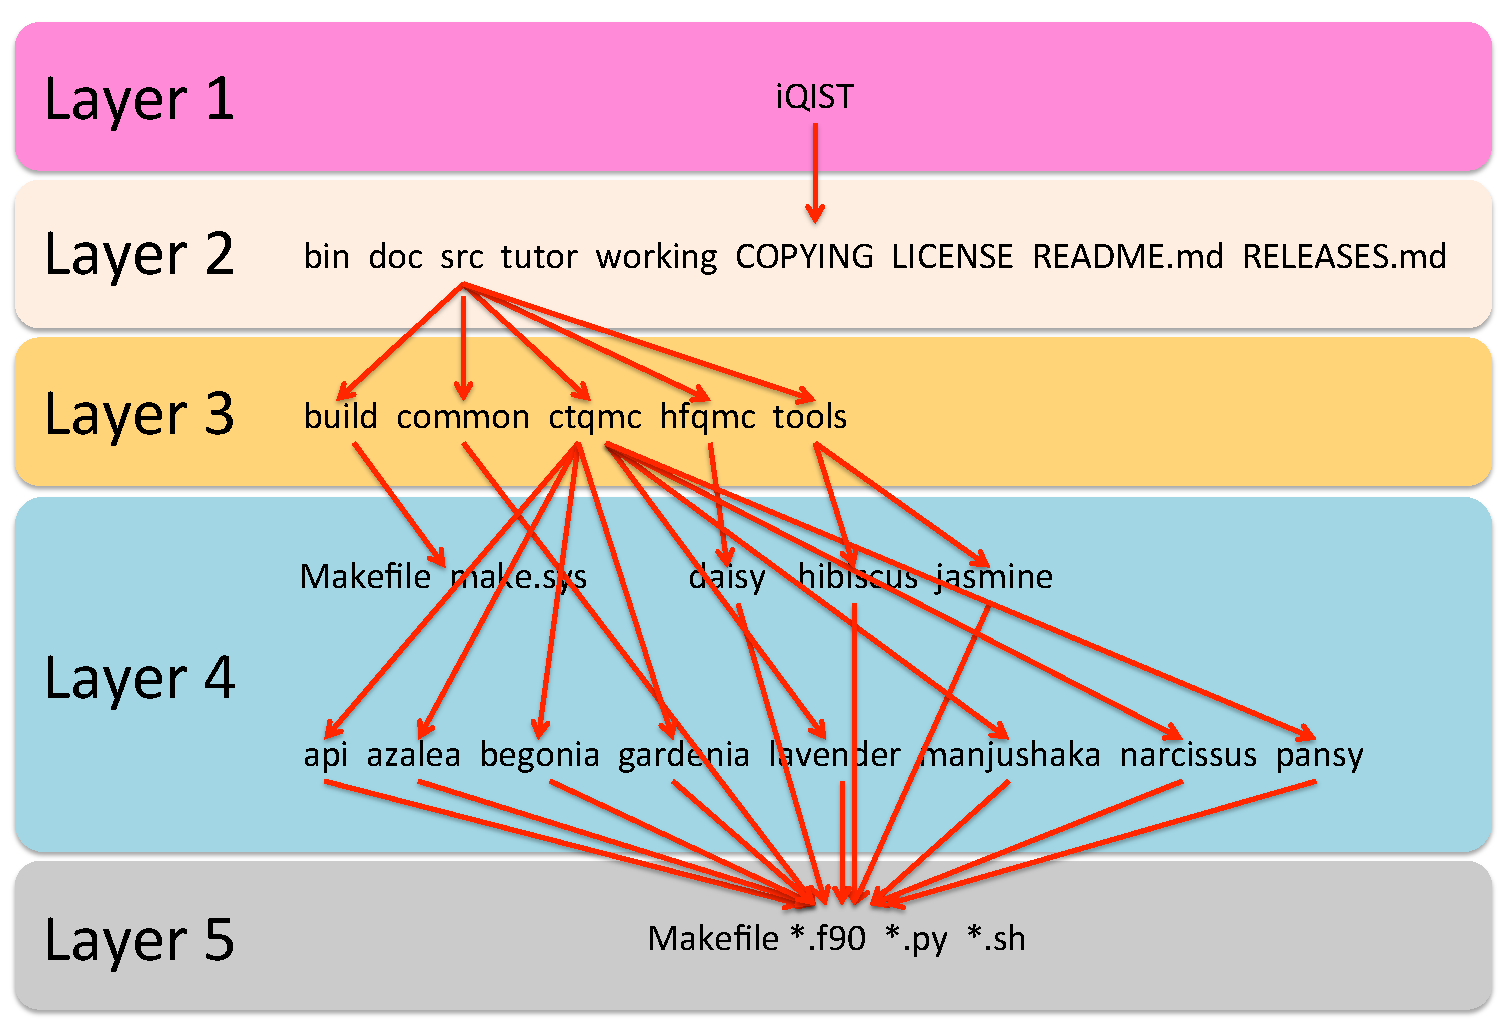
\includegraphics[scale=0.6]{figure/dir.pdf}
\caption{The directory structure of {\iqist} software package.\label{fig:dir}}
\end{figure}
The directory structure of the {\iqist} software package is shown in Fig.~\ref{fig:dir}.

COPYING: GNU General Public License Version 3.

LICENSE: Copyright declaration.

README.md: Readme.

RELEASES.md: Release notes.

iqist/bin: Used to save the executable programs.

iqist/doc: Documentation. The reference manual is in the manual directory. The document in the chinese directory is a bit outdated and will be removed in the future.

iqist/src: All of the source codes are here.

iqist/tutor: Tutorial materials are here.

iqist/working: Collection of typical input files which are used to benchmark {\iqist}.

Now let's make a dive into the iqist/src directory.

iqist/src/build: Top Makefile is here.

iqist/src/common: Common Service Subroutine Library (CSSL) and Common Service Module Library (CSML).

iqist/src/ctqmc/api: Application Programming Interface (API) for CT-QMC impurity solver.

iqist/src/ctqmc/azalea: The {\azalea} component.

iqist/src/ctqmc/begonia: The {\begonia} component.

iqist/src/ctqmc/gardenia: The {\gardenia} component.

iqist/src/ctqmc/lavender: The {\lavender} component.

iqist/src/ctqmc/manjushaka: The {\manjushaka} component.

iqist/src/ctqmc/narcissus: The {\narcissus} component.

iqist/src/ctqmc/pansy: The {\pansy} component.

iqist/src/hfqmc/daisy: The {\daisy} component.

iqist/src/tools/hibiscus: The {\hibiscus} component.

iqist/src/tools/jasmine: The {\jasmine} component.

\section{Compiling environment}

In order to compile and install {\iqist} correctly, you should ensure the following softwares are correctly installed and configured in your OS.

\underline{Fortran Compiler}

Most of the {\iqist}'s components are written in Fortran 90 language, so in order to compile {\iqist}, you need a Fortran 90 compiler. The components in {\iqist} can be successfully compiled using a recent Intel Fortran compiler. In fact, during the development of {\iqist}, we always used the Intel Fortran compiler. We can not guarantee that it can be compiled successfully by the other Fortran compilers, such as gfortran, PGI Fortran compiler, etc.

\underline{MPI}

All of the CT-QMC and HF-QMC impurity solvers in {\iqist} are fully parallelized with MPI. In order to obtain 
parallelized versions of quantum impurity solvers, some kinds of MPI implementations must be installed beforehand. Most of the MPI implementations, such as MPICH, MVAPICH, OpenMPI and Intel MPI are compatible with {\iqist}.

\underline{BLAS}

The {\iqist} depends on the BLAS library. As for the BLAS implementation, we strongly recommend OpenBLAS. The GotoBLAS2 is somewhat outdated and is not maintained any more, so we do not recommend it.

\underline{LAPACK}

The {\iqist} depends on the LAPACK library. For the LAPACK, the Intel Math Kernel Library is a good candidate. Of course, it is also possible to use the linear algebra library provided by the operating system, for example, the vecLib Framework in the Mac OS X.

\underline{Python}

Some post-processing scripts contained in the {\hibiscus} component are developed using the Python language. In order to execute these scripts or use the Python language binding for {\iqist}, the users should install Python 2.x. Furthermore, the newest numpy, scipy, and f2py packages are also necessary.

\section{Compiling system}

We use the make utility to build the {\iqist} software package. If you go through the directory structure of {\iqist}, you can find many Makefiles in different directories (for examples, iqist/src/ctqmc/api and iqist/src/hfqmc/daisy directories). For a given directory, if there is a Makefile in it, then you can always input the "make" command to build the code, the "make clean" command to clean binary objects, the "make clean-dat" command to clean the data files in it.

The top Makefile is in the iqist/src/build directory. In this directory, once you input the "make" command, a menu will be displayed in the terminal. Then you can follow the instructions to select suitable building jobs. In this directory, there is also a make.sys file which is used to configure the whole compiling system. Before you type any "make" commands, you have to edit the make.sys file at first to setup the compiling environment correctly. At least, you must setup the Fortran compiler, MPI compiler, BLAS and LAPACK libraries manually. All of the Makefile files depend on this make.sys. So be careful.

Next, we will explain the options in the make.sys file in details:

{\color{red}F90    = mpif90}

Intel Fortran compiler. It can be 'mpif90' or 'ifort'. If it is mpif90, the internal compiler invoked by mpif90 must be ifort.

{\color{red}LINKER = \$(F90)}

Linker. Here it is the same with compiler. Do not change it.

{\color{red}ARCHIVER = ar -ruv}

Archiver. It is used to pack the objects into a library. Do not modify it for ever.

{\color{red}MPI    = -DMPI}

Specify whether MPI is enable. If you want to compile a sequential code, please comment it out with '\#' symbol and then setup F90 to 'ifort'. We strongly suggest to compile MPI parallelized codes.

{\color{red}OMP    = \#-openmp}

Specify whether OpenMP is enable. If you want to disable it, please
comment it out. In default it is disabled. So far OpenMP was not used
by any components.

{\color{red}API    = \#-DAPI -DF2PY}

Specify whether we want to obtain a library version of {\iqist}. If it is enabled, what you can obtain is a library and you can write python or fortran codes to use it, instead of a standard executable program. At default it is disabled. If only the API macro is defined, the Fortran API will be generated. If both the API and F2PY macros are defined, the Python API and (slightly different) Fortran API will be generated. If only the F2PY macro is defined, it is invalid.

{\color{red}FPP    = -fpp}

Specify whether the fortran preprocessor (FPP) is used. It must be enabled or else the {\iqist} can not be compiled correctly.

{\color{red}CPP    = \$(FPP) \$(MPI) \$(OMP) \$(API)}

Collection of preprocessor directives. Do not modify it unless you are an expert of {\iqist}.

{\color{red}GPROF  = \#-pg}

Specify whether the code profiling should be done. If it is enabled, then after the code is finished, a gmon.out file will be generated. You can use the gprof tool to analyze the runtime information and find out the hotspot of the code. It is not wise to enable it to build a production code, because it will decrease the efficiency greatly.

{\color{red}CHECK  = -warn all \#-check all -traceback -g}

Used to specify what types of check should be done. '-warn all' means the check is done in compiling. '-check all' means the check will be done in running. '-traceback' enable us to track the exact position (line number and file name) where the error occurs. '-g' enable the compiler to generate debug information and embed them into the final program. Note that '-check all', '-traceback', and '-g' opinions will decrease the efficiency greatly.

{\color{red}CDUMP  = -vec-report2 -openmp-report2 -nogen-interfaces}

Specify whether the compiler will output useful optimization information in compiling.

{\color{red}LEVEL  = -O3 -xHost -unroll-aggressive -align all}

Collection of optimization opinions. '-O3' means the highest optimization. '-xHost' enables the compiler to generate the most suitable code for the current computer architecture. '-unroll-aggressive' means using aggressive method to unroll the loop structures. '-align all' means to align the arrays, structures, etc. Please modify them only if you are an expert of Intel Fortran Compiler and you know what you are doing.

{\color{red}MARCH  = -march=corei7-avx \# core2 corei7 corei7-avx core-avx-i core-avx2}

Used to specify the instruction sets that the current system can support. 'core2' is the safest choice and it works always. But it may be not the best. Please modify it only when you understand what you are doing.

{\color{red}FFLAGS = -c \$(CPP) \$(CHECK) \$(CDUMP) \$(LEVEL) \$(MARCH) \$(GPROF)}

Collection of Fortran compiler opinions. Do not modify them for ever.

{\color{red}LFLAGS = -static -Wl,-no\_pie \$(OMP) \$(GPROF)}

Collection of linker opinions. '-Wl,-no\_pie' is useful when you are using Mac Os X system. Do not modify them unless you know what you are doing.

{\color{red}LIBS   = -L/opt/intel/mkl/lib -lmkl\_core -lmkl\_sequential -lmkl\_rt}

Specify the external libraries. Now the {\iqist} software package depends on LAPACK and BLAS heavily. To achieve good performance, the highly optimized LAPACK and BLAS implementations are essential. Here we want to recommend the OpenBLAS and Intel MKL.

{\color{red}MPIL   = -L/usr/local/openmpi/lib -lmpi\_mpifh}

Specify the external mpi libraries for fortran binding. It is useful when you are compiling the python application programming interface using f2py (pyiqist and pydaisy). The f2py will automatically use the 'bare' intel fortran compiler (ifort) to link and generate the python modules (*.so). If you do not specify MPIL, then the python modules will not work properly. 

\section{Build full {\iqist} at one step}
Please change your current directory to iqist/src/build, and then enter the following command:

\noindent\colorbox{pink}{\parbox[r]{\linewidth}{\quad \$ make all}}

After a few minutes (depending on the performance of compiling platform), the {\iqist} is ready for use. Note that all of the executable programs will not be copied into the iqist/bin directory automatically. Please change your current directory to iqist/bin, and then enter the following command:

\noindent\colorbox{pink}{\parbox[r]{\linewidth}{\quad \$ ./setup.sh}}

Finally, do not forget to add this directory into the system environment variable PATH.

\section{Build common library}

Almost all of the components depend on CSSL and CSML, so you have to build them at first. Please change your current directory to iqist/src/build, and then enter the following command:

\noindent\colorbox{pink}{\parbox[r]{\linewidth}{\quad \$ make common}}

Or you can change your current directory to iqist/src/common, and then enter the following command:

\noindent\colorbox{pink}{\parbox[r]{\linewidth}{\quad \$ make}}

\section{Build application programming interface}

All of the CT-QMC impurity solvers components depend on the application programming interface (api), so you have to build it before you start to build individual CT-QMC impurity solver. Please change your current directory to iqist/src/build, and then enter the following command:

\noindent\colorbox{pink}{\parbox[r]{\linewidth}{\quad \$ make api}}

Or you can change your current directory to iqist/src/ctqmc/api, and then enter the following command:

\noindent\colorbox{pink}{\parbox[r]{\linewidth}{\quad \$ make}}

\section{Build quantum impurity solvers}

If you only want to build the quantum impurity solvers only, it is so easy. Please change your current directory to iqist/src/build, and then enter the following command:

\noindent\colorbox{pink}{\parbox[r]{\linewidth}{\quad \$ make solver}}

If you only want to build a specific quantum impurity solver, such as azalea, please enter the following commands:

\noindent\colorbox{pink}{\parbox[r]{\linewidth}{\quad \$ make azalea}}

Or you can change your current directory to iqist/src/ctqmc/azalea, and then enter the following command:

\noindent\colorbox{pink}{\parbox[r]{\linewidth}{\quad \$ make}}


\section{Build auxiliary tools}
\section{Build library for Fortran}
\section{Build module for Python}
\section{Build documents}
